%% fig_quarticrank.tex   (generated by make_round21.py; do not edit by hand)
%% The rank of the criterion at a quartic CM field (thm:quarticrank): the fifteen allowed points of the plane of the Hankel part and of R_1 + R_2, each with its value; filled points are reached with rho_1 = rho_2 (cor:quarticleast).
\documentclass[tikz,border=8pt]{standalone}
\usepackage{amsmath,amssymb}
\usetikzlibrary{arrows.meta,calc,decorations.pathreplacing}
%% palette.tex -- shared colour definitions for the figures
\definecolor{PInk}{RGB}{26,32,44}
\definecolor{PBlue}{RGB}{37,82,139}
\definecolor{PTeal}{RGB}{23,127,125}
\definecolor{POchre}{RGB}{193,138,44}
\definecolor{PClay}{RGB}{178,74,58}
\definecolor{PSlate}{RGB}{108,122,137}
\definecolor{PViolet}{RGB}{110,86,150}
\definecolor{WBlue}{RGB}{223,234,246}
\definecolor{WTeal}{RGB}{220,238,236}
\definecolor{WOchre}{RGB}{250,240,218}
\definecolor{WClay}{RGB}{247,229,224}
\definecolor{WSlate}{RGB}{238,241,244}
\definecolor{PMag}{RGB}{158,58,110}
\definecolor{PGrass}{RGB}{62,124,66}
\definecolor{PAmber}{RGB}{214,112,38}
\definecolor{PIndigo}{RGB}{58,64,140}
\definecolor{PRule}{RGB}{176,186,197}

%% shared macros so the standalone figures match the paper
\providecommand{\QQ}{\mathbb{Q}}
\providecommand{\ZZ}{\mathbb{Z}}
\providecommand{\RR}{\mathbb{R}}
\providecommand{\CC}{\mathbb{C}}
\providecommand{\PP}{\mathbb{P}}
\providecommand{\Kx}{K^{\times}}
\providecommand{\HW}{W}
\providecommand{\Nm}{\mathrm{N}}
\providecommand{\Hdg}{\mathrm{Hdg}}
\providecommand{\NS}{\mathrm{NS}}
\providecommand{\cA}{\mathcal{A}}
\providecommand{\cD}{\mathcal{D}}
\providecommand{\cF}{\mathcal{F}}
\providecommand{\cP}{\mathcal{P}}
\providecommand{\cO}{\mathcal{O}}
\providecommand{\cQ}{\mathcal{Q}}
\providecommand{\bbar}[1]{\overline{#1}}
\providecommand{\ch}{\operatorname{ch}}
\providecommand{\End}{\mathrm{End}}
\providecommand{\Ext}{\operatorname{Ext}}
\providecommand{\Supp}{\operatorname{Supp}}

\begin{document}
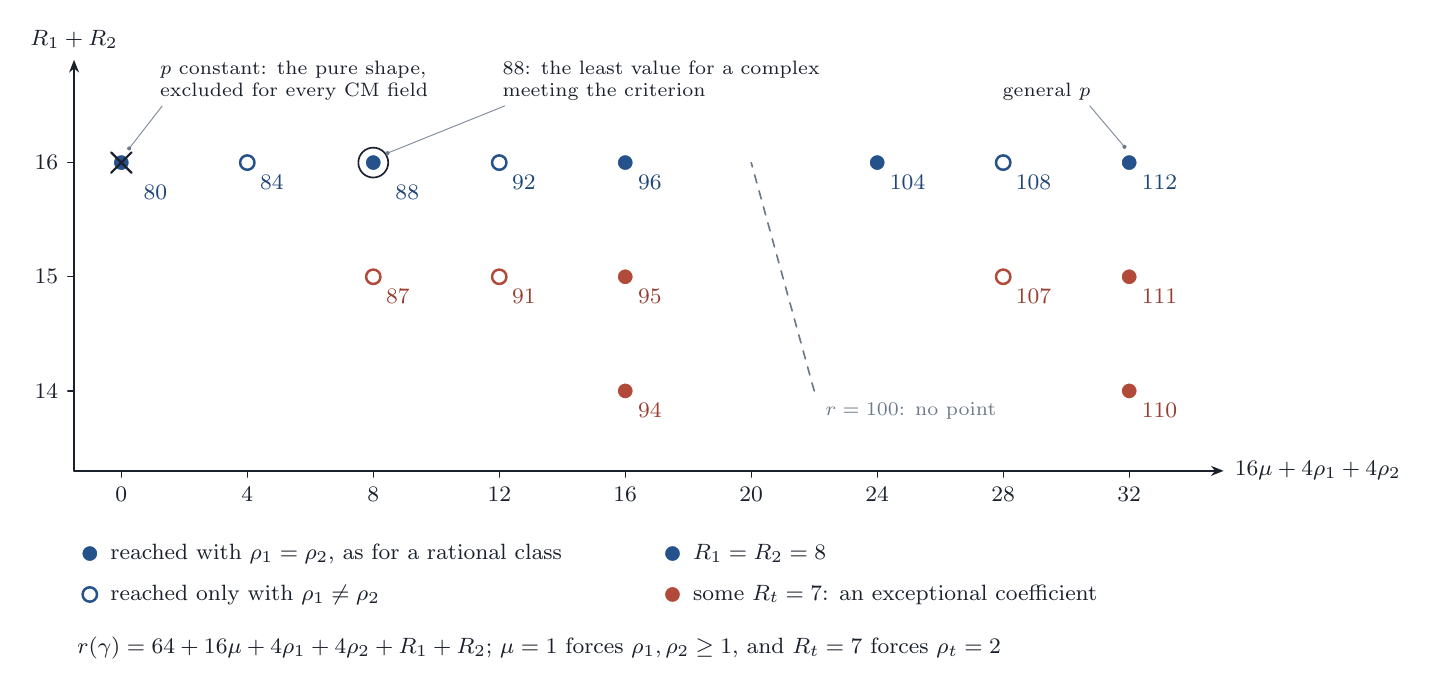
\begin{tikzpicture}[x=1cm,y=1cm,line join=round,line cap=round,
  font=\small,text=PInk,lbl/.style={inner sep=1pt}]
  \draw[PInk,line width=0.55pt,-{Stealth[length=4.6pt,width=3.6pt]}] (-0.6000,0.0000) -- (14.0000,0.0000);
  \draw[PInk,line width=0.55pt,-{Stealth[length=4.6pt,width=3.6pt]}] (-0.6000,0.0000) -- (-0.6000,5.2200);
  \draw[PInk,line width=0.45pt] (0.0000,0.0000) -- (0.0000,-0.0800);
  \draw[PInk,line width=0.45pt] (1.6000,0.0000) -- (1.6000,-0.0800);
  \draw[PInk,line width=0.45pt] (3.2000,0.0000) -- (3.2000,-0.0800);
  \draw[PInk,line width=0.45pt] (4.8000,0.0000) -- (4.8000,-0.0800);
  \draw[PInk,line width=0.45pt] (6.4000,0.0000) -- (6.4000,-0.0800);
  \draw[PInk,line width=0.45pt] (8.0000,0.0000) -- (8.0000,-0.0800);
  \draw[PInk,line width=0.45pt] (9.6000,0.0000) -- (9.6000,-0.0800);
  \draw[PInk,line width=0.45pt] (11.2000,0.0000) -- (11.2000,-0.0800);
  \draw[PInk,line width=0.45pt] (12.8000,0.0000) -- (12.8000,-0.0800);
  \draw[PInk,line width=0.45pt] (-0.6000,1.0150) -- (-0.6800,1.0150);
  \draw[PInk,line width=0.45pt] (-0.6000,2.4650) -- (-0.6800,2.4650);
  \draw[PInk,line width=0.45pt] (-0.6000,3.9150) -- (-0.6800,3.9150);
  \draw[PSlate,line width=0.6pt,dashed] (8.8000,1.0150) -- (8.0000,3.9150);
  \path[fill=PBlue,draw=white,line width=0.60pt] (0.0000,3.9150) circle (3.00pt);
  \path[fill=white,draw=PBlue,line width=0.90pt] (1.6000,3.9150) circle (2.60pt);
  \path[fill=white,draw=PClay,line width=0.90pt] (3.2000,2.4650) circle (2.60pt);
  \path[fill=PBlue,draw=white,line width=0.60pt] (3.2000,3.9150) circle (3.00pt);
  \path[fill=white,draw=PClay,line width=0.90pt] (4.8000,2.4650) circle (2.60pt);
  \path[fill=white,draw=PBlue,line width=0.90pt] (4.8000,3.9150) circle (2.60pt);
  \path[fill=PClay,draw=white,line width=0.60pt] (6.4000,1.0150) circle (3.00pt);
  \path[fill=PClay,draw=white,line width=0.60pt] (6.4000,2.4650) circle (3.00pt);
  \path[fill=PBlue,draw=white,line width=0.60pt] (6.4000,3.9150) circle (3.00pt);
  \path[fill=PBlue,draw=white,line width=0.60pt] (9.6000,3.9150) circle (3.00pt);
  \path[fill=white,draw=PClay,line width=0.90pt] (11.2000,2.4650) circle (2.60pt);
  \path[fill=white,draw=PBlue,line width=0.90pt] (11.2000,3.9150) circle (2.60pt);
  \path[fill=PClay,draw=white,line width=0.60pt] (12.8000,1.0150) circle (3.00pt);
  \path[fill=PClay,draw=white,line width=0.60pt] (12.8000,2.4650) circle (3.00pt);
  \path[fill=PBlue,draw=white,line width=0.60pt] (12.8000,3.9150) circle (3.00pt);
  \draw[PInk,line width=0.8pt] (-0.1300,3.7850) -- (0.1300,4.0450);
  \draw[PInk,line width=0.8pt] (-0.1300,4.0450) -- (0.1300,3.7850);
  \path[fill=none,draw=PInk,line width=0.60pt] (3.2000,3.9150) circle (5.40pt);
  \path[fill=PBlue,draw=white,line width=0.60pt] (-0.4000,-1.0500) circle (3.00pt);
  \path[fill=white,draw=PBlue,line width=0.90pt] (-0.4000,-1.5700) circle (2.60pt);
  \path[fill=PBlue,draw=white,line width=0.60pt] (7.0000,-1.0500) circle (3.00pt);
  \path[fill=PClay,draw=white,line width=0.60pt] (7.0000,-1.5700) circle (3.00pt);
  \draw[PSlate!85,line width=0.35pt] (0.5200,4.6350) -- (0.1000,4.0950);
  \fill[PSlate] (0.1000,4.0950) circle (0.75pt);
  \draw[PSlate!85,line width=0.35pt] (4.8700,4.6350) -- (3.3800,4.0350);
  \fill[PSlate] (3.3800,4.0350) circle (0.75pt);
  \draw[PSlate!85,line width=0.35pt] (12.3000,4.6350) -- (12.7400,4.1150);
  \fill[PSlate] (12.7400,4.1150) circle (0.75pt);
  \node[lbl,anchor=north,text=PInk,font=\footnotesize] at (0.0000,-0.1600) {$0$};
  \node[lbl,anchor=north,text=PInk,font=\footnotesize] at (1.6000,-0.1600) {$4$};
  \node[lbl,anchor=north,text=PInk,font=\footnotesize] at (3.2000,-0.1600) {$8$};
  \node[lbl,anchor=north,text=PInk,font=\footnotesize] at (4.8000,-0.1600) {$12$};
  \node[lbl,anchor=north,text=PInk,font=\footnotesize] at (6.4000,-0.1600) {$16$};
  \node[lbl,anchor=north,text=PInk,font=\footnotesize] at (8.0000,-0.1600) {$20$};
  \node[lbl,anchor=north,text=PInk,font=\footnotesize] at (9.6000,-0.1600) {$24$};
  \node[lbl,anchor=north,text=PInk,font=\footnotesize] at (11.2000,-0.1600) {$28$};
  \node[lbl,anchor=north,text=PInk,font=\footnotesize] at (12.8000,-0.1600) {$32$};
  \node[lbl,anchor=east,text=PInk,font=\footnotesize] at (-0.7600,1.0150) {$14$};
  \node[lbl,anchor=east,text=PInk,font=\footnotesize] at (-0.7600,2.4650) {$15$};
  \node[lbl,anchor=east,text=PInk,font=\footnotesize] at (-0.7600,3.9150) {$16$};
  \node[lbl,anchor=west,text=PInk,font=\footnotesize] at (14.1000,0.0000) {$16\mu+4\rho_{1}+4\rho_{2}$};
  \node[lbl,anchor=south,text=PInk,font=\footnotesize] at (-0.6000,5.3200) {$R_{1}+R_{2}$};
  \node[lbl,anchor=west,text=PSlate,font=\scriptsize] at (8.9000,0.7662) {$r=100$: no point};
  \node[lbl,anchor=west,text=PBlue!85!black,font=\footnotesize] at (0.2400,3.5422) {$80$};
  \node[lbl,anchor=west,text=PBlue!85!black,font=\footnotesize] at (1.7200,3.6622) {$84$};
  \node[lbl,anchor=west,text=PClay!85!black,font=\footnotesize] at (3.3200,2.2122) {$87$};
  \node[lbl,anchor=west,text=PBlue!85!black,font=\footnotesize] at (3.4400,3.5422) {$88$};
  \node[lbl,anchor=west,text=PClay!85!black,font=\footnotesize] at (4.9200,2.2122) {$91$};
  \node[lbl,anchor=west,text=PBlue!85!black,font=\footnotesize] at (4.9200,3.6622) {$92$};
  \node[lbl,anchor=west,text=PClay!85!black,font=\footnotesize] at (6.5200,0.7622) {$94$};
  \node[lbl,anchor=west,text=PClay!85!black,font=\footnotesize] at (6.5200,2.2122) {$95$};
  \node[lbl,anchor=west,text=PBlue!85!black,font=\footnotesize] at (6.5200,3.6622) {$96$};
  \node[lbl,anchor=west,text=PBlue!85!black,font=\footnotesize] at (9.7200,3.6622) {$104$};
  \node[lbl,anchor=west,text=PClay!85!black,font=\footnotesize] at (11.3200,2.2122) {$107$};
  \node[lbl,anchor=west,text=PBlue!85!black,font=\footnotesize] at (11.3200,3.6622) {$108$};
  \node[lbl,anchor=west,text=PClay!85!black,font=\footnotesize] at (12.9200,0.7622) {$110$};
  \node[lbl,anchor=west,text=PClay!85!black,font=\footnotesize] at (12.9200,2.2122) {$111$};
  \node[lbl,anchor=west,text=PBlue!85!black,font=\footnotesize] at (12.9200,3.6622) {$112$};
  \node[lbl,anchor=west,text=PInk,font=\scriptsize,align=left] at (0.4500,4.9571) {$p$ constant: the pure shape,\\excluded for every CM field};
  \node[lbl,anchor=west,text=PInk,font=\scriptsize,align=left] at (4.8000,4.9571) {$88$: the least value for a complex\\meeting the criterion};
  \node[lbl,anchor=east,text=PInk,font=\scriptsize] at (12.3500,4.8165) {general $p$};
  \node[lbl,anchor=west,text=PInk,font=\footnotesize] at (-0.1800,-1.0500) {reached with $\rho_{1}=\rho_{2}$, as for a rational class};
  \node[lbl,anchor=west,text=PInk,font=\footnotesize] at (-0.1800,-1.5700) {reached only with $\rho_{1}\ne\rho_{2}$};
  \node[lbl,anchor=west,text=PInk,font=\footnotesize] at (7.2200,-1.0500) {$R_{1}=R_{2}=8$};
  \node[lbl,anchor=west,text=PInk,font=\footnotesize] at (7.2200,-1.5700) {some $R_{t}=7$: an exceptional coefficient};
  \node[lbl,anchor=west,text=PInk,font=\footnotesize] at (-0.6000,-2.2528) {$r(\gamma)=64+16\mu+4\rho_{1}+4\rho_{2}+R_{1}+R_{2}$; $\mu=1$ forces $\rho_{1},\rho_{2}\ge1$, and $R_{t}=7$ forces $\rho_{t}=2$};
\end{tikzpicture}
\end{document}
